\section{Strategy Pattern}
\label{sec:oop:strategy:pattern}

  Ya deberían empezar a ver el problema en el que nos estamos metiendo.
  Cada vez que queramos agregar una nueva carta mágica, tendremos que crear una nueva subclase de
  \texttt{AbstractMagicCard} y agregar un nuevo método \texttt{useOn(Player)}.
  Muchas cartas tendrán efectos similares, así que vamos a poder aprovechar la herencia para no
  repetir tanto código, pero a medida que el problema se va complejizando, por ejemplo, si ahora 
  queremos agregarle efecto a otros tipos de cartas, como las cartas trampa o monstruo, vamos a 
  tener que los mismos efectos (o variaciones de los mismos) en distintos tipos de cartas.

  Una manera de resolver este problema es utilizando el principio de \textit{composition over
  inheritance} que dice que las clases debieran poder lograr un comportamiento polimórfico a través
  de la composición de otras clases en lugar de la herencia.
  En este caso, en lugar de crear una jerarquía de clases que represente las cartas, vamos a crear
  una jerarquía de clases que represente los efectos de las cartas.

  \begin{defaultbox}[Strategy Pattern]
    \textbf{Problema:} Tenemos clases relacionadas que se diferencian solamente en su 
    comportamiento.

    \textbf{Solución:} Extraer el comportamiento que varía a una clase separada y hacer que las
    clases que se diferencian se compongan de la clase que contiene el comportamiento que varía.
  \end{defaultbox}

  El patrón Strategy es un patrón de diseño de comportamiento que nos permite definir una familia
  de algoritmos, encapsular cada uno de ellos y hacer que los algoritmos sean intercambiables dentro
  de un objeto.

  La \cref{fig:oop:strategy:pattern} muestra la estructura del patrón Strategy.

  \begin{figure}[ht]
    \centering
    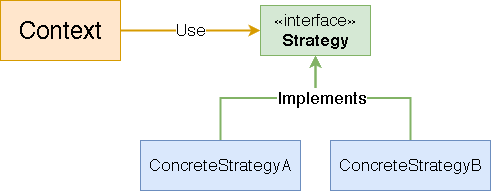
\includegraphics[width=0.5\textwidth]{img/oop/strategy/strategy_pattern.png}
    \caption{Estructura del patrón Strategy}
    \label{fig:oop:strategy:pattern}
  \end{figure}

